\documentclass[border=1pt]{standalone}
% Shared preamble for standalone figures in this directory.
% Compile with XeLaTeX from 讲义/figs, or via the figures target.
\usepackage{ctex}
\usepackage{amsmath}
\usepackage{amssymb}
\usepackage{bm}
\usepackage{mathtools}
\usepackage{tikz}
\renewcommand{\vec}[1]{\boldsymbol{#1}}
\newcommand{\cC}{\mathcal{C}}
\newcommand{\cD}{\mathcal{D}}
\newcommand{\R}{\mathbf{R}}
\usetikzlibrary{
    arrows.meta,
    calc,
    decorations.markings,
    angles,
    quotes,
    positioning,
    patterns,
    shapes.geometric
}

\begin{document}
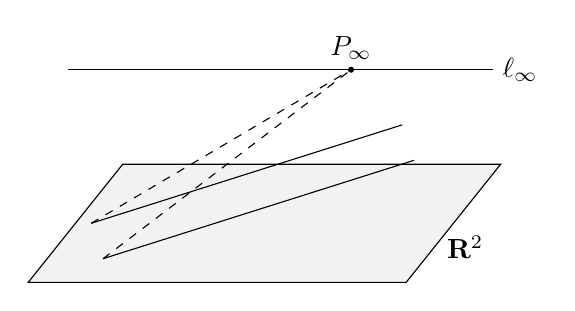
\begin{tikzpicture}[scale=1.0, >=Stealth]
    \draw[fill=gray!10] (0,0) -- (4.8,0) -- (6,1.5) -- (1.2,1.5) -- cycle;
    \node at (5.55,0.45) {$\R^2$};
    \draw (0.5,2.7) -- (5.9,2.7);
    \node[right] at (5.9,2.7) {$\ell_\infty$};
    \coordinate (I) at (4.1,2.7);
    \draw[dashed] (0.95,0.3) -- (I);
    \draw[dashed] (0.8,0.75) -- (I);
    \draw (0.95,0.3) -- (4.9,1.55);
    \draw (0.8,0.75) -- (4.75,2.0);
    \fill (I) circle (1.1pt) node[above] {$P_\infty$};
\end{tikzpicture}

\end{document}
